\subsubsection{RimWorld}
Das Strategiespiel \textit{RimWorld} ist ein im Jahr 2018 erschienenes Sci-Fi \textit{Colony Management} Game und wurde von \textit{Ludeon Studios} entwickelt und publiziert. Im normalen Szenario startet man mit drei Überlebenden eines Raumschiffabsturzes und versucht seine Kolonie aufzubauen und am Leben zu halten. Das Spiel hat etliche Mechaniken und Tücken, und durch den \textit{AI Storyteller}, welcher eine Vielfalt an Events plant und durchführt, ist eine hohe \textit{replayability} gegeben. Dieser kann auf eine gewünschte Schwierigkeit gestellt werden, von friedfertig bis unfair. Nachdem man den gewünschten Storyteller ausgewählt hat kann man den Planeten generieren (vgl. \autoref{image:rimworld}) und seinen Startpunkt innerhalb der Spielwelt bestimmen (vgl. \autoref{image:rimworld2}).

\begin{figure}
    \begin{center}
        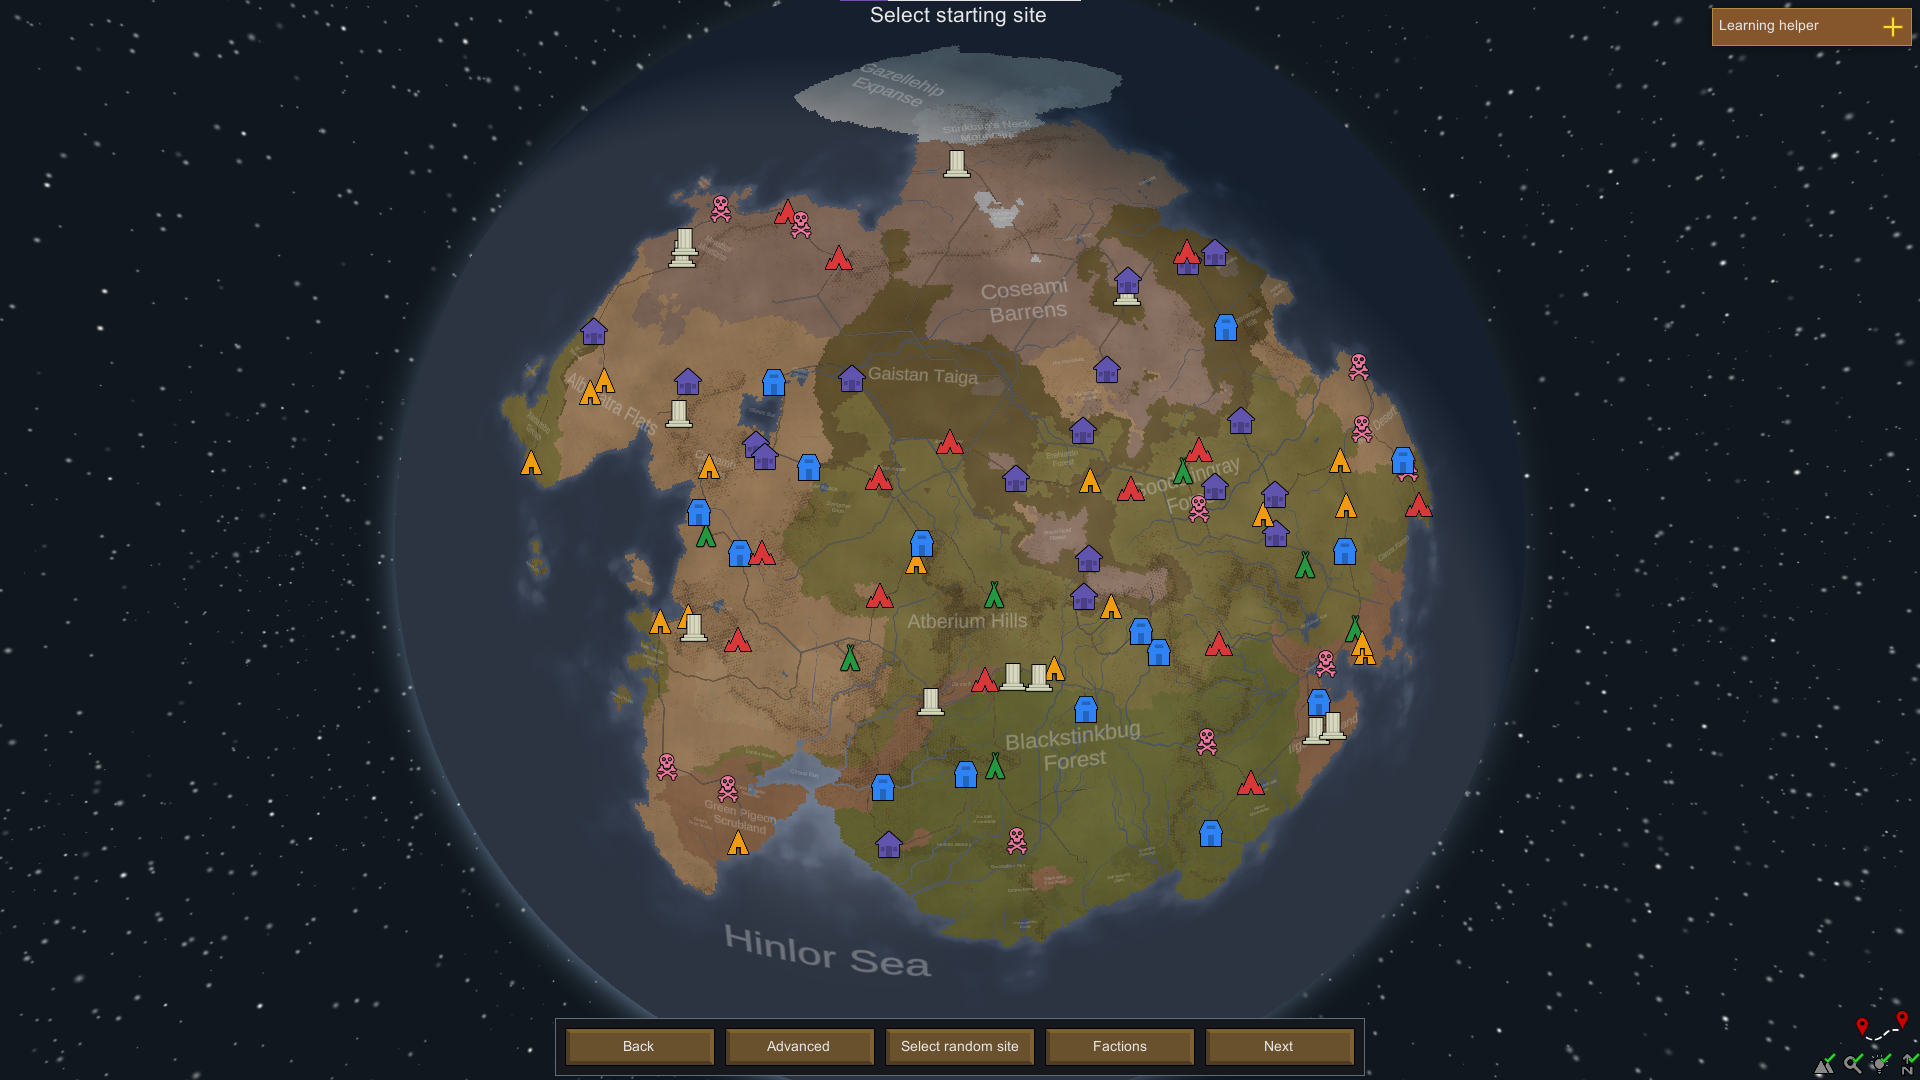
\includegraphics[width=300px]{0.bilder/rimworld.png}
    \end{center}
    \caption{Generierter Planet, Screenshot aus RimWorld} \label{image:rimworld}
\end{figure}

\begin{figure}
    \begin{center}
        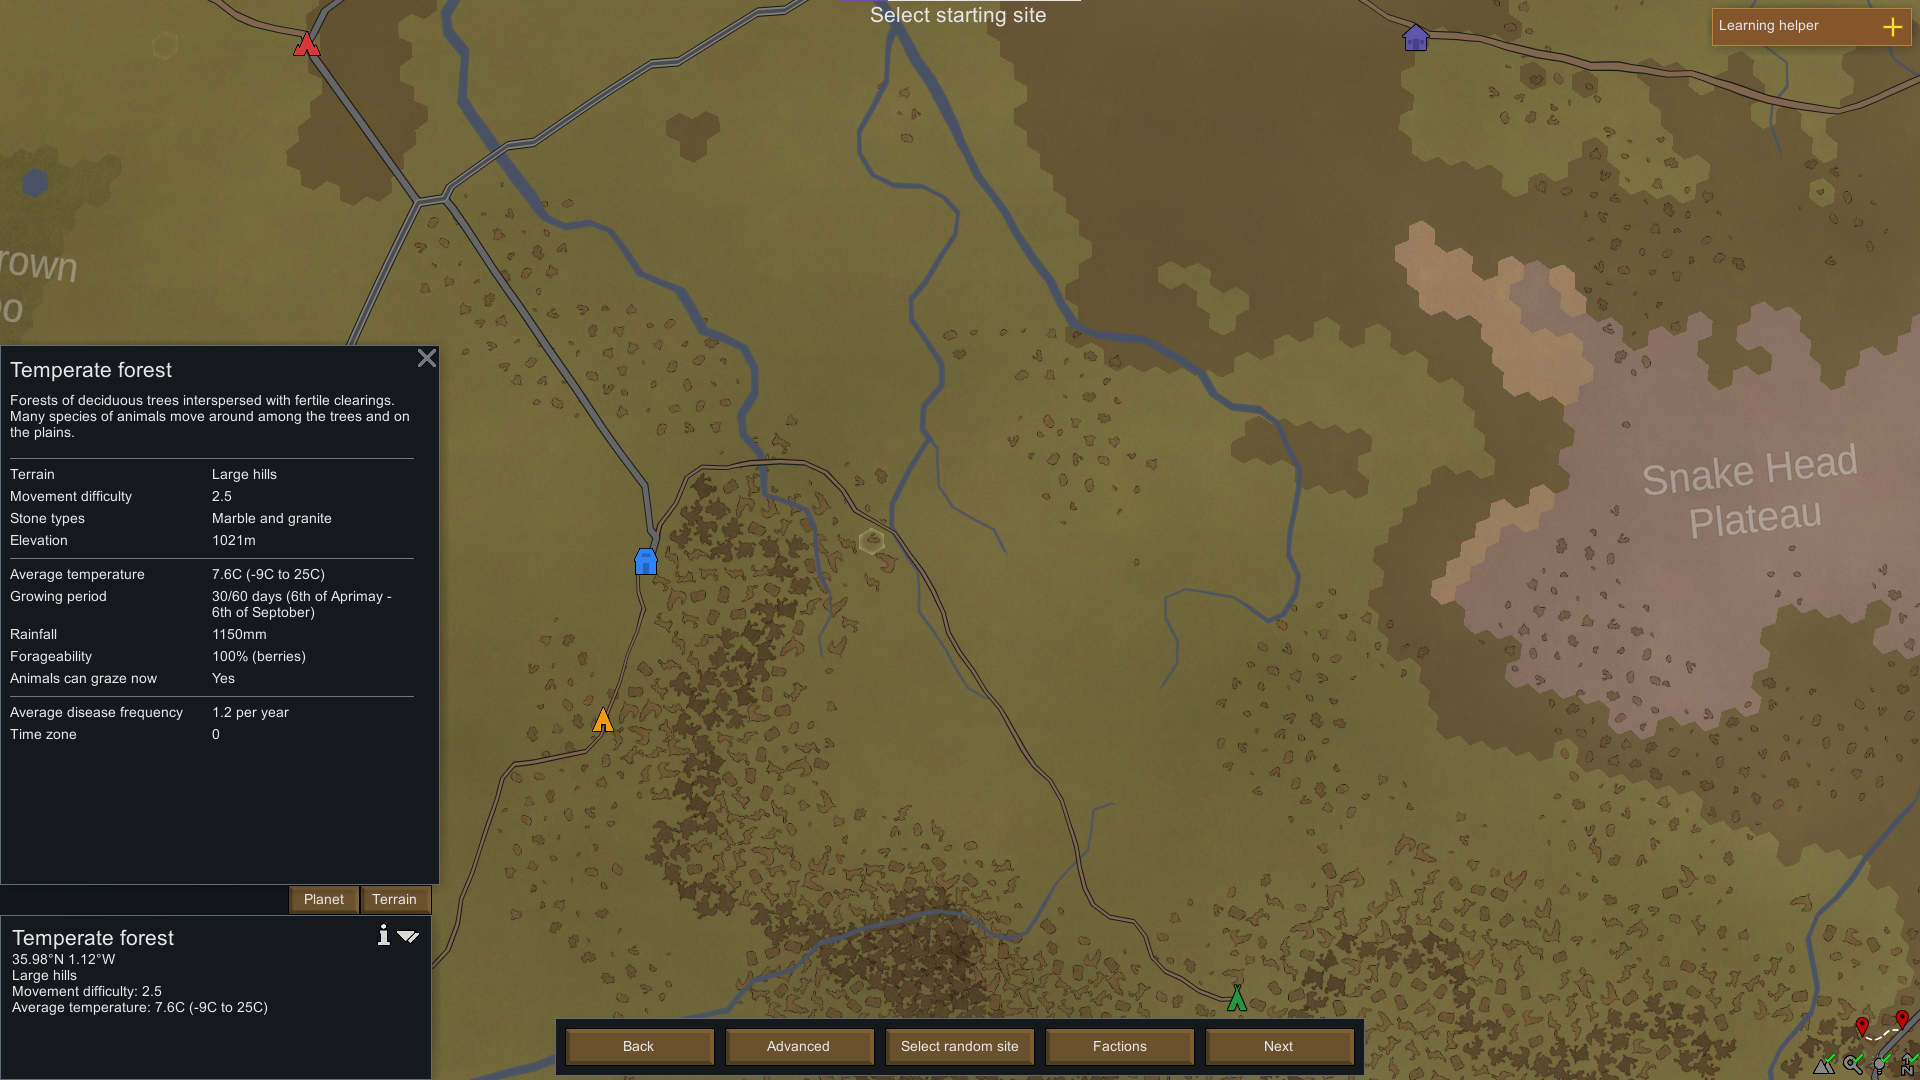
\includegraphics[width=300px]{0.bilder/rimworld2.png}
    \end{center}
    \caption{Ausgewählter Startpunkt für die Kolonie, Screenshot aus RimWorld} \label{image:rimworld2}
\end{figure}

\newparagraph{Spielwelt}
Die Welt ist für gewöhnlich eine Pangaea-artige Landmasse auf einem dreidimensionalen, blauen Planeten mit einem Äquator und einem Pol (vgl. \autoref{image:rimworld}). Der Planet ist aufgeteilt in hexagonale Kacheln, welche jeweils eine Karte symbolisieren. Die Kacheln haben dabei jeweils verschiedene Eigenschaften, die dann auf der gesamten Karte, welche der Spieler aussucht, gelten. Auf \autoref{image:rimworld2} lassen sich am linken Rand die meisten Eigenschaften anzeigen. Darunter die Terrain-Eigenschaften, wie viel Berge es gibt und damit auch Erzquellen, welche Steinarten es gibt und die Höhe der Karte. Außerdem ist ein maßgeblicher Faktor die Extreme der Temperaturen, zu welchen Zeiten man Felder anbauen kann und wie viel Regen für gewöhnlich fällt. Der Name der Kacheln, in diesem Fall \glqq Temperate Forest\grqq, gibt außerdem Aufschluss darüber, wie bewaldet die Kachel ist. Je nach Distanz zum Pol oder Äquator ändern sich diese Eigenschaften. Außerdem besitzen manche Kacheln einen Fluss oder bestehen gänzlich aus Wasser oder Eis, oder haben eine Anbindung zu einer Straße (grau) oder einem Feldweg (braun). Wählt man eine Kachel aus und drückt auf \glqq Next\grqq am unteren Bildschirmrand, gelangt man in die Auswahl der Kolonisten.

\newparagraph{Kolonisten}
Das Herz des Spielgeschehens sind die Kolonisten, die, mit manchen Ausnahmen, ihre zugewiesenen Aufgaben erfüllen. Die drei Startkolonisten kann man so lange neu generieren, bis man zufrieden ist. Es gibt dabei mehrere Eigenschaften, die ein Kolonist mit sich bringt. Die darunter fundamentalsten Eigenschaften sind die \textit{Skills}, welche mittig in \autoref{image:rimworldcharacter} zu sehen sind. Es gibt 12 verschiedene Skills, wovon jeder Kolonist ein bestimmtes Level hat. Diese werden zwischen \textit{0 - 5} generiert, wonach noch die \textit{Hintergründe} (engl. \textit{backstories}) und \textit{Eigenschaften} (engl. \textit{traits}) der jeweiligen Kolonisten addiert werden \cite*[]{rimworld:colonist}. Manche Hintergründe addieren oder subtrahieren Level von Skills, manche machen manche Tätigkeiten und damit einhergehende Skills auch unmöglich, darunter der Hintergrund \textit{Romanschriftsteller} (engl. \textit{novelist}), welcher es dem Kolonisten unmöglich macht, einfache Arbeiten zu erledigen, etwa Putzen oder Gegenstände umhertragen \cite*[]{rimworld:backstories}. Eigenschaften sind analog zu den Hintergründen zufällig generiert, beziehen sich größtenteils jedoch auf soziale Interaktionen oder bringen bestimmte Boni oder Mali für die \textit{Stimmung} des Kolonisten, darunter Sexualitäten, wie schnell der Kolonist lernen kann, oder exotischere Eigenschaften wie \textit{Kannibale} oder \textit{Psychopath} \cite*[]{rimworld:traits}. Die Flammen neben dem Level der Skills stehen für die \textit{Passion} des Kolonisten für bestimmte Skills. Ist keine Flamme neben dem Level zu sehen, so lernt der Kolonist diese Fähigkeit beim Durchführen davon mit einem Faktor von \textit{35\%}. Ist eine Flamme vorhanden, ist der Kolonist \textit{interessiert} und hat einen Lernfaktor von \textit{100\%}. Sind zwei Flammen vorhanden, \textit{brennt} der Kolonist für diese Tätigkeit und lernt mit einem Faktor von \textit{150\%}. Da viele verschiedene Tätigkeiten zu bestimmten Zeitpunkten ausschlaggebend für das Überleben der Kolonie sein könnten, kann es sinnvoll sein, eine breite Palette verschiedener Passionen und hochrangigen Skills zu haben. Ältere Kolonisten haben für gewöhnlich höhere Skills, sind jedoch davon öfter von \textit{Gesundheitsproblemen} betroffen, etwa Verlust von Seh- und Hörvermögen, oder langsamere Laufgeschwindigkeit. Außerdem haben manche Startkolonisten bereits zuvor gebildete \textit{Beziehungen} zu manch anderen, welche bestimmte Interaktionen vereinfachen oder erschweren.
 
\begin{figure}
    \begin{center}
        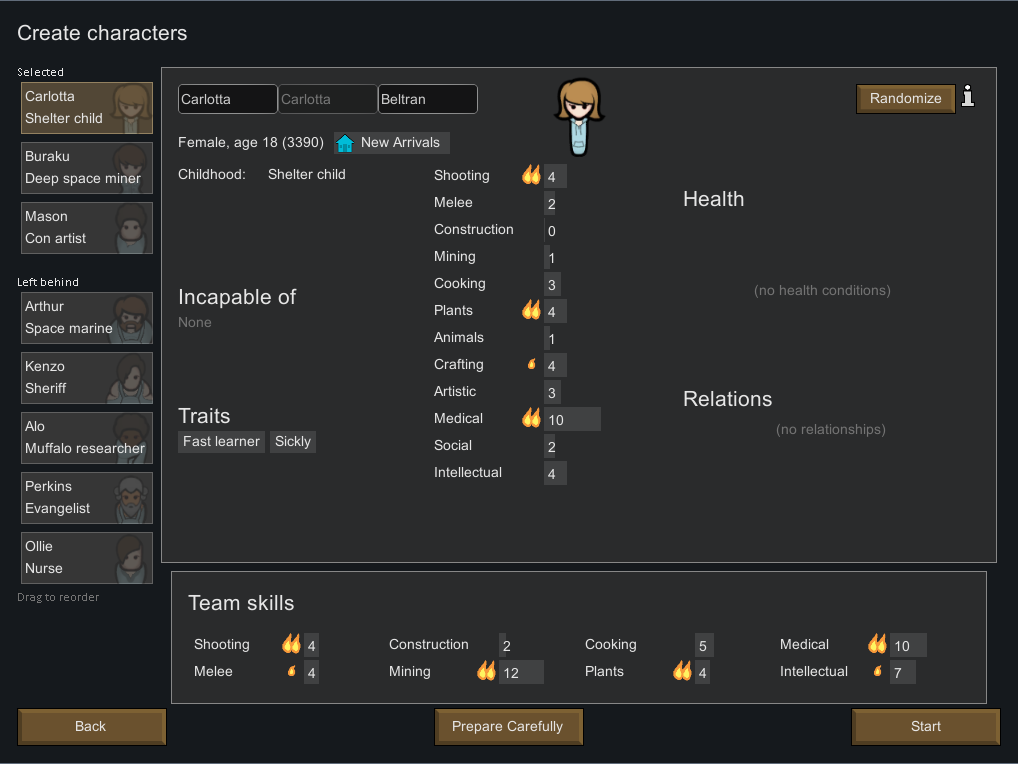
\includegraphics[width=300px]{0.bilder/rimworldcharacter.png}
    \end{center}
    \caption{Auswahl der Startkolonisten, Screenshot aus RimWorld} \label{image:rimworldcharacter}
\end{figure}

\newparagraph{Spielgeschehen}
Der Spieler wird nach der Anfangssequenz des Absturzes der Kolonisten nicht an die Hand genommen. Ein großer Teil des Spieles besteht darin, Strategien für das Überleben der Kolonie zu finden. Für gewöhnlich beginnt man damit, erste Teile der zukünftigen Basis zu bauen, wie diese aussehen soll und aus welchem Material diese besteht ist, wie so oft in diesem Spiel, dem Spieler selbst überlassen. Jeder Kolonist hat eine \textit{Stimmung} (engl. \textit{mood}), welche es gilt im Auge zu behalten (vgl. \autoref{image:rimworldmood}). Sollte die Stimmung zu lange zu niedrig sein, wird der Kolonist in einen nicht kontrollierbaren Zustand fallen, auch engl. \textit{mental break} genannt, wovon es verschiedene gibt. Darunter \textit{tantrum}, wobei der Kolonist alle möglichen Gebäude und Strukturen in seiner Sichtweite attackiert und möglicherweise zerstört, oder \textit{given up and leaving}, wobei der Kolonist die Spielerkolonie verlässt und aus dem Spiel entfernt wird \cite*[]{rimworld:mentalbreak}. Um diese Zustände zu vermeiden muss der Spieler sinnvoll die zu Anfang gegebenen Ressourcen nutzen, und für Nahrung, Unterschlupf, Wärme, Licht und etliche weitere Gegebenheiten sorgen. Je nach gewählten AI Storyteller passieren selten oder öfter Events, welche das Spielgeschehen maßgeblich beeinflussen können. Darunter sind \textit{raids}, wobei fremde Kolonien die Spielerkolonie angreifen, Gebäude zerstören, Reichtümer stehlen oder Kolonisten verschleppen, oder ein zufälliger Ansturm an Biebern, welche sämtliche Bäume auf der Karte Stück für Stück abholzen \cite*[]{rimworld:events}. Um gegebene Probleme zu Lösen kann der Spieler neue Technologien erforschen, welche letztendlich bis zum Bau eines Raumschiffes führen, was das vorprogrammierte Endziel des Spiels ist. Auf dem Weg zum Bau des Raumschiffes wird der Spieler also konstant vor neue Probleme, Launen der Kolonisten und Ressourcenmanagement gestellt, wodurch eine hohe replayability gegeben ist.

\begin{figure}
    \begin{center}
        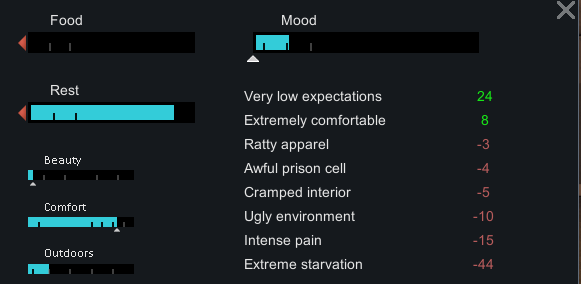
\includegraphics[width=300px]{0.bilder/rimworldmood.png}
    \end{center}
    \caption{Stimmungsbalken und -einflüsse, Screenshot aus RimWorld} \label{image:rimworldmood}
\end{figure}

\newparagraph{User Interface}
Das UI von RimWorld ist sehr voll, in jeder Ecke des Bildschirms finden sich direkt mehrere verschiedene Informationen, welche der Spieler erst kennenlernen und verstehen muss. Im Folgenden wird sich stark auf \autoref{image:rimworldui} berufen, anhand dessen das UI analysiert wird. Das UI ist zum besseren Verständnis in 13 verschiedene Stücke aufgeteilt, welche allesamt eigene Funktionen und einen bestimmten Mehrwert bieten. 

\begin{figure}
    \begin{center}
        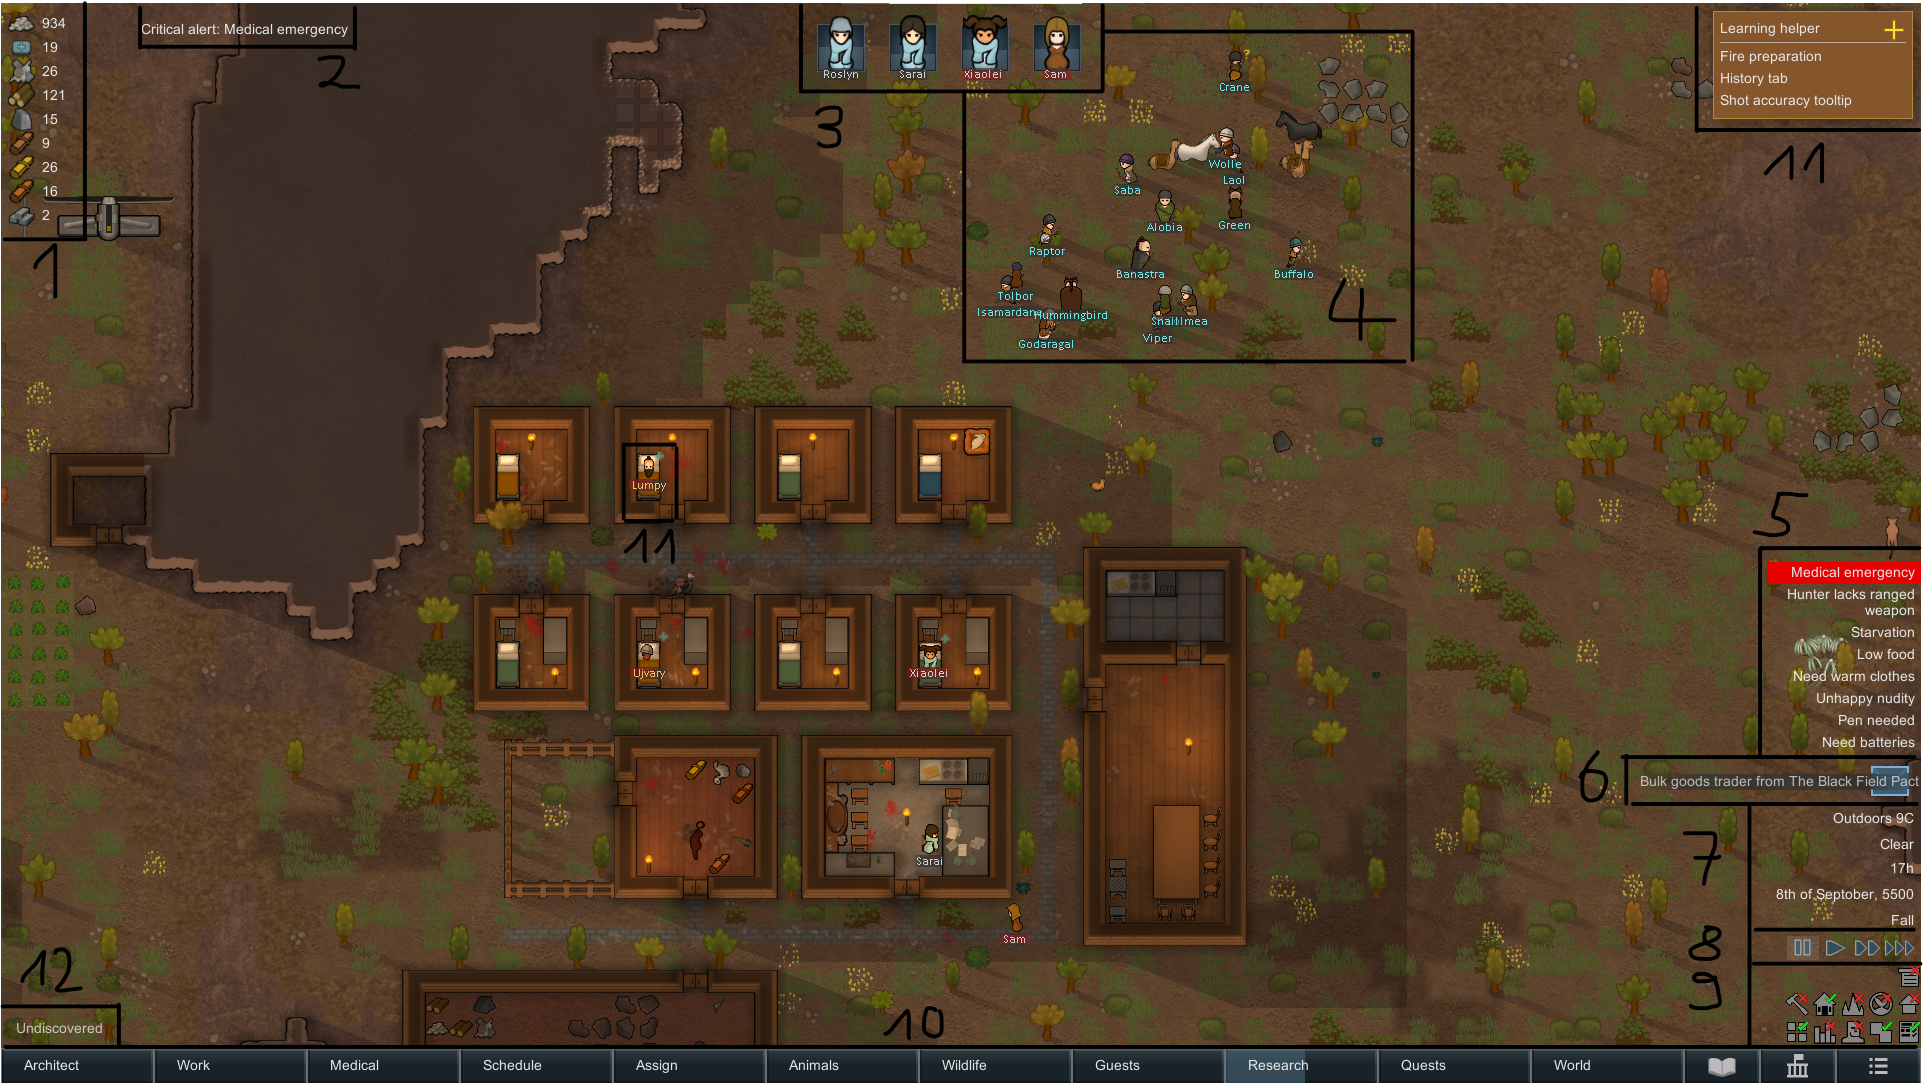
\includegraphics[width=400px]{0.bilder/rimworldui.png}
    \end{center}
    \caption{User Interface, Screenshot aus RimWorld} \label{image:rimworldui}
\end{figure}

Der erste Bereich des UI (1) zeigt die Ressourcen im Besitz des Spielers. Nicht alle Ressourcen werden vom Spieler besessen, sondern erst jene, die im definierten Lager vorhanden sind.
Der zweite Bereich (2) ist für kritische Meldungen, die sofortiges Handeln erfordern, in diesem Fall ein medizinischer Notfall, welcher zum Tod des Kolonisten führen kann.
In Bereich (3) werden alle Kolonisten, die Teil der eigenen Kolonie sind, angezeigt. Man kann dort sowohl Namen, als auch Aussehen, derzeitige Lebenspunkte und momentane Stimmung ablesen (hellblaue Füllung im Hintergrund des Quadrats).
Im vierten Bereich (4) ist gerade ein Event zu sehen, welches zufällig generiert wurde. In diesem Fall wird die Spielerkolonie von einer Händlerkarawane besucht, welche ein eigenes Inventar hat und mit dem Spieler handeln kann, also auch ein \textit{Händler} im Sinne einer ökonomischen Funktion.
Bereich (5) zeigt einige Zustände der Spielerkolonie an, darunter derzeitig hungernde Kolonisten, oder dass ein Jäger keine Waffe zum Jagen besitzt. Sehr dringende Zustände mit sofortigem Handlungsbedarf werden, wie in der Grafik zu erkennen, rot hinterlegt dargestellt.
In Bereich (6) werden ausschließlich vom AI Storyteller generierte Events mitgeteilt, also Hitzewellen, Angriffe oder, wie in diesem Fall, Besuche von Händlerkarawanen.
Im siebten Bereich (7) erkennt man meteorologische Informationen zu derzeitigen Wettergegebenheiten, der Temperatur, den derzeitigen Monat und die Jahreszeit.
Bereich (8) beinhaltet die Elemente zur Steuerung der Spielgeschwindigkeit.
Bereich (9) zeigt verschiedene Optionen zum Anzeigen bestimmter Informationen. Man kann sich beispielsweise noch die Fruchtbarkeitsgrade des Bodens einblenden lassen, oder die Schönheit der Umgebung aus der Sicht eines Kolonisten.
Der zehnte Bereich (10) stellt die Menüleiste dar, unter welcher man die meisten Aktionen im Spiel durchführen kann. Unter dem Reiter \textit{Architect} finden sich zum Beispiel Möbel und Strukturen (vgl. \autoref{image:rimworlduimenu}), welche man platzieren kann. Der am besten passende Kolonist wird dann dieser Tätigkeit zugeordnet.



\begin{figure}
    \begin{center}
        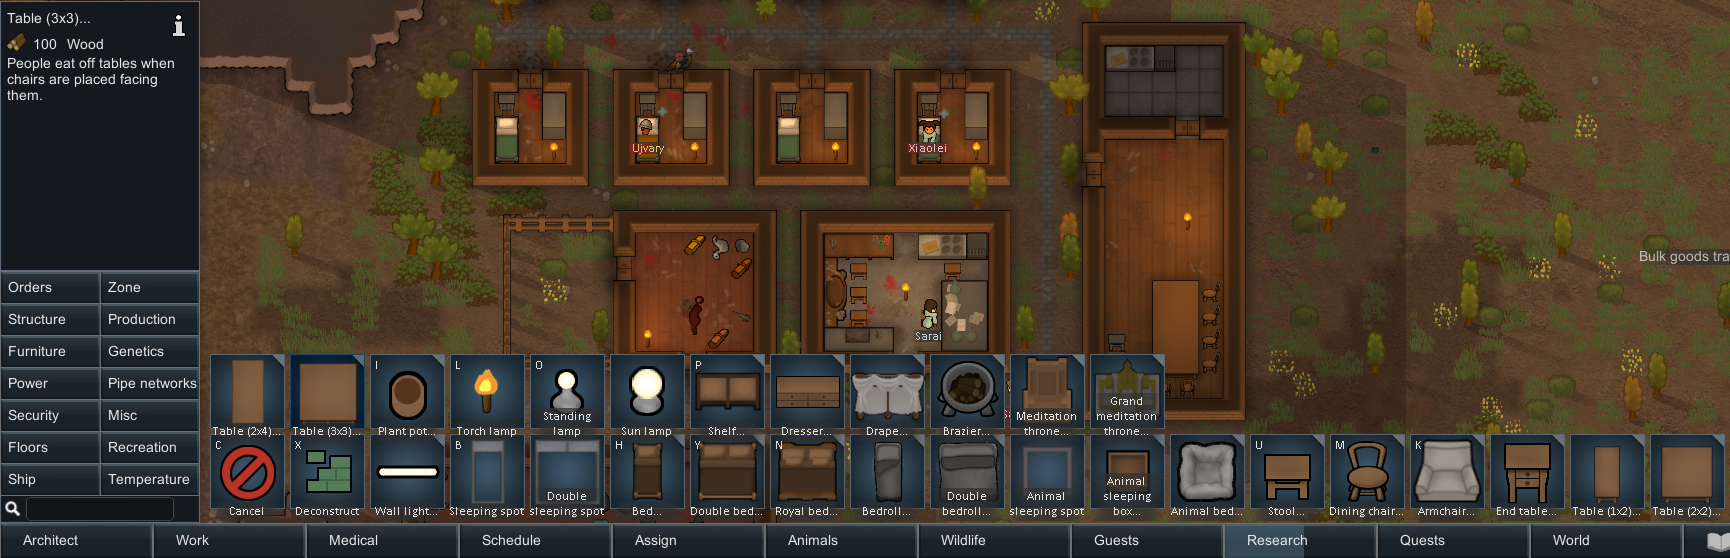
\includegraphics[width=400px]{0.bilder/rimworlduimenu.png}
    \end{center}
    \caption{Baumenü, Screenshot aus RimWorld} \label{image:rimworlduimenu}
\end{figure}